\subsubsection{Fully Connected layer} \label{subs:fcl}
The perceptron described in Section \ref{subs:perceptron} can be considered as a linear classifier for which the decision boundary is the hyperplane, as seen in equation \eqref{eq:linearclassifer} \cite{matteucci_artificial_2019}.
%
\begin{equation}
    b + w_1 \cdot x_1 + ... + w_{n_{in}} \cdot x_{n_{in}} = 0
    \label{eq:linearclassifer}
\end{equation}
%
\begin{figure}
    \centering
    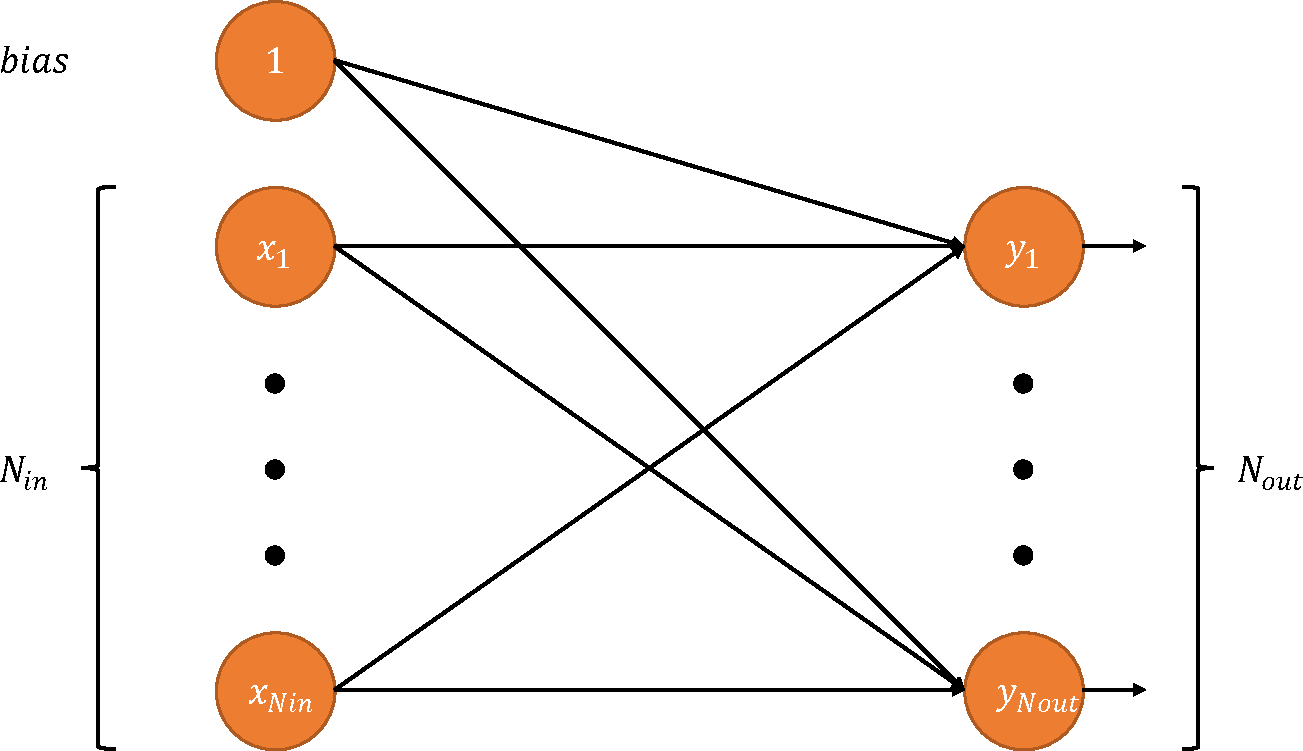
\includegraphics[width=\textwidth]{fcl.pdf}
    \caption{A fully connected layer}
    \label{fig:fcn}
\end{figure}
%
The perceptron is therefore limited because is has only linear decision boundary. It means that it is possible to implement the AND and OR boolean functions with perceptron but impossible to learn the XOR function for example \cite{minsky_perceptrons_1969}. In order to be able to build non-linear models, a topology of perceptrons needs to be used \cite{khan_survey_2020}. It is composed of layers of perceptrons called fully-connected layer in \acrshort{cnn}. This layer is represented on Figure \ref{fig:fcn}. It can be seen that each perceptron is connected either to the inputs either to the perceptrons of the previous layers.

A fully-connected layer is characterized by the number of neurons, activation functions, and the values of weights. The output vector $\boldsymbol{y}$ is defined by equation \eqref{eq:fcn}, where $\boldsymbol{x}$ is the vector of the input of the layer and $x_0 = 1$ is the bias; $\boldsymbol{w}$ is the vector of all the weights of the layer ($w^i_*$ are the weights of the ith perceptron and $w^*_0$ are the biases); $h$ is the activation function of the layer \cite{abdelouahab_accelerating_2018}.
%
\begin{equation}
    \boldsymbol{y} = h(\boldsymbol{w}^T \boldsymbol{x}) \qquad \Leftrightarrow \qquad \forall o \in \{ 1, ..., N_{out} \} : y_o = h(\sum^{N_{in}}_{i=0} w^o_i \cdot x_i)
    \label{eq:fcn}
\end{equation}
%
As we have seen that perceptrons can be used to construct a non-linear classifier, we see in the next section \ref{subs:2dconv} the main operation in the \acrshort{cnn}: the \textbf{convolution}, which extracts the feature from input images.
